\subsection{TET Histograms and Distance}
	Comparing the TET can be done in different ways. One of the methods that can be used to find similarity between the TETs is to transform the TETs into histograms and compare these\cite{JAEGER201330}. By counting the number of each type of subTET we can calculate each substructure's percentile distribution for \autoref{fig:Tetekempel}, by dividing the number of subTET in a specific type by the total number of subTETs. The simple TET in \autoref{Eq:TETvector} would give a representation as \autoref{fig:Tethistogram}.
	
	\begin{figure}[H]
		\centering
		\begin{adjustbox}{width=0.5\textwidth}
			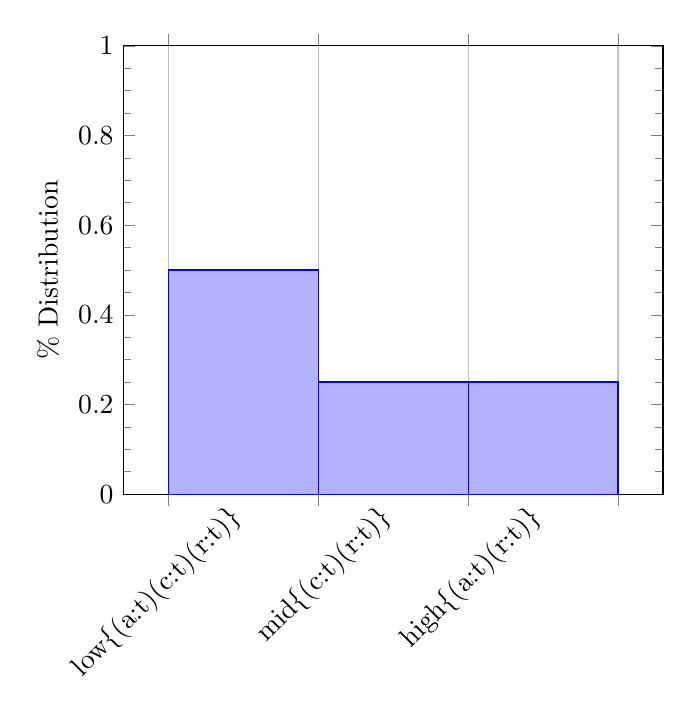
\begin{tikzpicture}
	\begin{axis}[
	ybar interval, 
	ymax=1,ymin=0, 
	minor y tick num = 3,
	ylabel = {\% Distribution},
	symbolic x coords={low\{(a:t)(c:t)(r:t)\}, mid\{(c:t)(r:t)\}, high\{(a:t)(r:t)\}, high\{(y:t)(r:t)\}},
	x tick label style={font=\normalsize, rotate=45, anchor=east},
	]
	\addplot coordinates {(low\{(a:t)(c:t)(r:t)\}, 0.5) (mid\{(c:t)(r:t)\}, 0.25) (high\{(a:t)(r:t)\}, 0.25) (high\{(y:t)(r:t)\}, 0.10)};
	\end{axis}
\end{tikzpicture}

%\begin{tikzpicture}

%\definecolor{bblue}{HTML}{4F81BD}

%\begin{axis}[
%major x tick style = transparent,
%ymin=0,
%bar width=1cm,
%minor y tick num = 3,
%ymajorgrids = true,
%ylabel = {\% distribution},
%symbolic x coords={low\{(a:t)(c:t)(r:t)\}, mid\{(c:t)(r:t)\}, high\{(a:t)(r:t)\}},
%xtick = data,
%x tick label style={font=\normalsize, rotate=45, anchor=east},
%]
%\addplot[ybar , style={bblue,fill=bblue,mark=none}]
%coordinates {(low\{(a:t)(c:t)(r:t)\}, 0.5) (mid\{(c:t)(r:t)\}, 0.25) (high\{(a:t)(r:t)\}, 0.25)};

%\end{axis}
%\end{tikzpicture}
		\end{adjustbox}
		\caption{The TET histogram derived from \autoref{fig:Tetekempel}}
		\label{fig:Tethistogram}
	\end{figure}
	
	By using this representation as a vector we can compare two histograms with simple distance measures as for example manhatten or euclidean distance.
	
	when comparing two histograms, one might have some elements that the other does not have. For any missing element in a histogram we add the value $0$, and we are thereby able to calculate distance for the missing element. A simple example done with manhatten distance can be seen in \autoref{Eq:manhattencomparason}\cite{singh2013k}.
	
	\begin{equation}\label{Eq:manhattencomparason}
	D(\begin{bmatrix}
	x_{1.1} \\
	x_{1.2} \\
	\end{bmatrix},
	\begin{bmatrix}
	x_{2.1} \\
	x_{2.2} \\
	x_{2.3}
	\end{bmatrix})= |x_{1.1} - x_{2.1}| + |x_{1.2} - x_{2.2}| + |0 - x_{2.3}|
	\end{equation}
	
	\autoref{Eq:manhattencomparason} is easily implemented if the vectors are represented as dictionaries. We can then go through the union of dictionary keys from the two dictionaries and return $0$ if a key is not found. The value $0$ will then be used in the calculation. 
